\documentclass[a4paper]{article}
    \usepackage[T1]{fontenc}
    \usepackage[utf8]{inputenc}
    \usepackage[italian]{babel}
    \usepackage{enumitem}
    \usepackage{graphicx}
    \usepackage{makecell}
    \graphicspath{{./images/}}
    \usepackage{tabularx}
    %\usepackage{geometry} 
    %\geometry{a4paper,top=3cm,bottom=3cm,left=3.5cm,right=3.5cm,% heightrounded,bindingoffset=5mm}
    
    \begin{document}
    
    \author{Manuel Trivilino, Davide Salaorni, Luca Terracciano}
    
    \title{\Large Data4Help\\
    \Large RASD Requirements Analysis and Specification Document
    }
    
    \maketitle
    \newpage
    
    \tableofcontents
    \newpage
    
    \section{Introduction}
    
    \subsection{Purpose}
    
    \subsection{Scope}
    
    \paragraph{Description of the given problem}
    
    \paragraph{}
    TrackMe is a company that develops software-based services for third parties and for consumers. The main service is called Data4Help.
     Data4Help is a service that allows third parties to monitor the location and the health status of individual, it handles a policy of permissions for each user and collects individual’s data from their personal devices.
    The service supports the registration of individuals who, by registering, agree that TrackMe acquires their data. After registration, these third parties can request:
    
    \begin{itemize}
        \item Access to the data of some specific individuals (we can assume, for instance, that they know an 
        individual by his/her social security number or fiscal code in Italy). In this case, TrackMe passes 
        the request to the specific individuals who can accept or refuse it.
        
        \item Access to anonymized data of groups of individuals (for instance, all those living in a certain 
        geographical area, all those of a specific age range, etc.). These requests are handled directly 
        by TrackMe that approves them if it is able to properly anonymize the requested data. For 
        instance, if the third party is asking for data about 10-year-old children living in a certain street 
        in Milano and the number of these children is two, then the third party could be able to derive 
        their identity simply having people monitoring the residents of the street between 8.00 and 
        9.00 when kids go to school. Then, to avoid this risk and the possibility of a misuse of data,
        TrackMe will not accept the request. For simplicity, we assume that TrackMe will accept any 
        request for which the number of individuals whose data satisfy the request is higher than 
        1000.
    
    \end{itemize}
    
    \paragraph{}
    As soon as a request for data is approved, TrackMe makes the previously saved data available to the 
    third party. Also, it allows the third party to subscribe to new data and to receive them as soon as 
    they are produced.
    TrackMe develops itself two third-party services: AutomatedSOS and Track4Run.
    
    \paragraph{Goals}
    
    \begin{enumerate}[label*={G.\arabic*}]
        
        %Data4Help
        
        \item Allow users to register in two different ways: single person and third parties.
        
        \item Third parties can request for anonymized data.
    
        \item Third parties can subscribe to the service in order to periodically receive new data.
            
        \item Third parties can receive for a individual user's data.
        
        %AutomatedSOS
        \item Users' health status is continuously checked in AutomatedSOS and in case of it overcomes a certain threshold values an ambulance is called within 5 seconds.
        
        %Track4Run
        \item Users can organize a run.
        \item Users can enroll to a run.
        \item Users can be spectators of a run seeing the partecipants' position on a map.
        
    \end{enumerate}
    
    \subsection{Definitions, Acronyms, Abbreviation}
    
    
    \subsection{Revision History}
    
    \subsection{Reference Documents}
    
    \subsection{Document Structure}
    
    \section{Overall Description}
    
    \subsection{Product Perspective}
    
    \begin{figure}[h!]
        \centering
        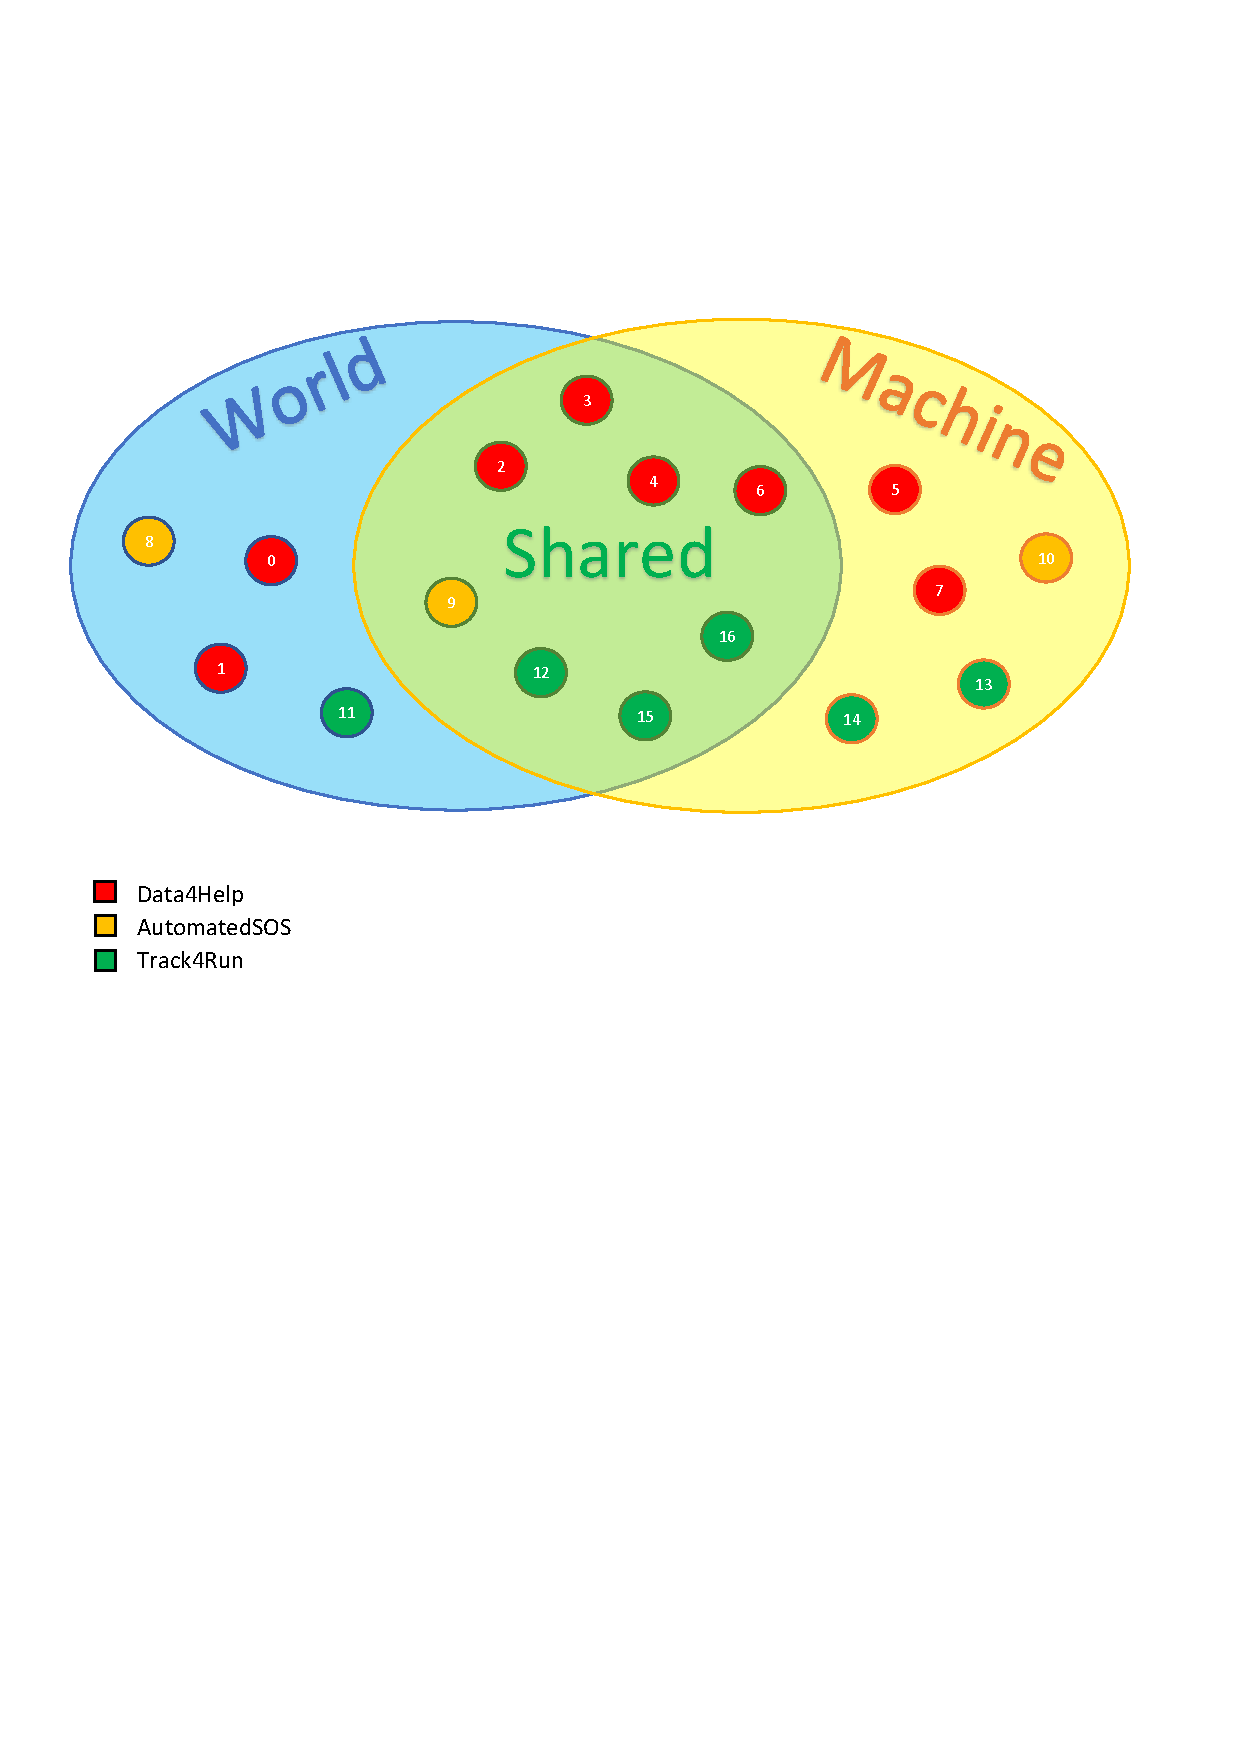
\includegraphics[width=\linewidth]{worldMachineShared-small}
        \caption{World, machine and shared phenomena.}
        \label{fig:my_label}
    \end{figure}
    
    
    \subsection{Product Functions}
    
    \subsection{User Characteristics}
    
    \paragraph{}The following actors are the users of the services offered by TrackMe. 
    
    
    \begin{itemize}
        \item User:  a person that is successfully registered to TrackMe as consumer and allow to acquire anonymous data, eventually a client of third party services (i.e. AutomatedSOS, Track4Run) that allows even personal data.
        
        \item Third Parties:  a company or a person who is registred to TrackMe as "Third party" that access to anonymous and can require to access to individual data.
        
    \end{itemize}
    
    \subsection{Assumption, Dependencies and Constraints}
    
    \subsubsection{Domain Assumptions}
    
    
    \begin{enumerate}[label={[D.\arabic*]}]
        
        \item The data collected from the devices (position and health status) are reliable, accurate and in real time.
        \item The personal information given by the user (age, address, gender...) are correct and the account is not used by other people. 
        \item Ambulance call and information about patients' status and position are correctly dispatched to the ambulance contact center.
        \item Information and data (places, maps, paths, etc.) received from external services are correct are reliable.
        
    \end{enumerate}
    
    
    \section{Specific Requirements}
    
    \subsection{External Interface Requirements}
    
    \subsubsection{User Interfaces}
    
    \subsubsection{Hardware Interfaces}
    
    \subsubsection{Software Interfaces}
    
    \subsubsection{Communication Interfaces}
    
    \subsection{Functional Requirements}
    
    \begin{enumerate}[label*=\bf{G.\arabic*}]
        
        %Data4Help
        
        \item \textbf{Allow users to register in two different ways: single person and third parties.}
        
        \begin{enumerate}
            \item [D.2] The personal informations given by the user (age, address, gender...) and the third parties are correct and the account is not used by other people. 
            \item [R.1] People can create a user account selecting username, password, giving personal informations (age, address,gender) and allow to share their anonymized data.
            \item [R.2] It is possible to create a third party account selecting username and password and giving the company main information.
        \end{enumerate}
        
        \item Third parties can receive anonymized data.
                
            \begin{enumerate}
                \item [R.3] Data4Help allows third parties to request anonymized data acquired from a filtered group of users (by age, gender, address, etc.).
                \item [R.4] Data4Help collects data from registered users and gives access to third parties only if the number of individuals whose data satisfy the request is higher than 1000.
                \item [D.2] The personal informations given by the user (age, address, gender...) and the third parties are correct and the account is not used by other people.
            \end{enumerate}
            
            
        \item Third parties can subscribe to the service in order to periodically receive new data.
        
        \begin{enumerate}
            \item [R.5] Data4Help allows third parties to join the subscription service for an indeterminate period and then, in case, unsubscribe from that.
            \item [R.6] Data4Help provides new data, checking each time if groups data satisfy the given constraint (number of individuals not lower than a thousand).
            \item [R.7] Data4Help keeps track of the associations between third parties subscriptions and the required group data.
        \end{enumerate}
        
        
        \item Third parties can receive specific person's data.
                
        \begin{enumerate}
                \item[R.8] Data4Help allows third parties to require specific person's data. 
                \item [R.9] Data4Help forwards requests from third parties to the demanded users which can accept or refuse to share their own personal data.
                \item [R.10] Data4Help keeps track of the connections between a specific user and the third parties which can access to his/her data.
                \item [R.11] Data4Help allows third parties to have access to demanded users' data each time they need them.
            \end{enumerate}
                
            
        %AutomatedSOS
        \item Users' health status is continuously checked in AutomatedSOS and if it is below a certain threshold values an ambulance is called within 5 seconds and sent to the user's position.
    
        \begin{enumerate}
            \item [D.1] The data collected from the devices (position and health status) are reliable, accurate and in real time.
            \item [R.12] Users' health and position information received by Data4Help are analyzed and compared with the threshold values.
            \item [R.13] In case of emergency (the health status values overcome the threshold) a request for an ambulance is sent to the ambulance dispatcher in 5 seconds, containing the user's information.
            \item [D.3] Ambulance call and information about patients' status and position are correctly dispatched to the ambulance contact center.
        \end{enumerate}
        
        %Track4Run
        \item Users can organize a run.
        
        \begin{enumerate}
            \item [R.14] Users select the day, the hour at which the run begins, the starting point, the ending point and the path for the run.
            \item [R.15] The run event is stored in the system in order to be managed during its lifecycle.
            \item [D.4] Information and data (places, maps, paths, etc.) received from external services are correct and reliable.
        \end{enumerate}
        
        \item Users can enroll to a run.
        
        \begin{enumerate}
            \item [R.16] Users can browse among the available runs and see their information.
            \item [R.17] Users can choose a run and register to it as a runners.
  % NON-FUNCTIONAL         \item [R.12] Users can choose to see the available runs filtering them by city and/or date. 
            \item [R.18] The system saves the enrolled users as runners and keeps track of the association with the run event.
        \end{enumerate}
        
        \item Users can be spectators of a run seeing the participants' position on a map.
        
        \begin{enumerate}
            \item [R.19] The system keeps track of all the enrolled runners' position during the run.
            \item [R.20] Users who require to watch a run are saved as spectators to the run event.
            \item [R.21] Track4Run offers the possibility to see the run live through a map.
        \end{enumerate}
        
    \end{enumerate}
    
    
    \paragraph{Use cases}

\subsubsection{User's sign up}
\begin{center}
    \begin{tabular}{ l || p{8cm} ||}
        \bf{ACTORS} & User \\ 
        \hline
        \bf{ENTRY CONDITIONS} & No entry condition needed  \\ 
        \hline
        \bf{EVENTS FLOW} & \begin{itemize}[noitemsep, topsep=0cm, leftmargin=*] \vspace{-0.2cm}
            \item[1.] User opens Data4Help app and press “Sign Up” button.
            \item[2.] User inserts personal informations (name, address, age, gender, fiscal code).
            \item[3.] User selects email and password.
            \item[4.] User allows terms of conditions to share anonymized data with Data4Help.
            \item[5.] User completes the registration.
            \item[6.] The system saves the new account.
        \end{itemize}\\ 
        \hline
        \bf{EXIT CONDITIONS} & The user is successfully registered and his/her data can be collected by Data4Help, he/she is redirected to the user page\\ \hline
        \bf{EXCEPTIONS} & \begin{itemize}[noitemsep, topsep=0cm, leftmargin=*] \vspace{-0.2cm}
            \item[1.] The user doesn’t fill all the mandatory fields with valid data.
            \item[2.]The inserted email is already used by another user.
            \item[3.] The user doesn’t allow the term of condition and he/she can’t complete the registration.
        \end{itemize}
        \\ \hline \hline
    \end{tabular}
\end{center}

\vspace{1cm}

\subsubsection{Request for anonymous data}
\begin{center}
    \begin{tabular}{l || p{8cm} ||}
        \bf{ACTORS} & Third Party \\ \hline
        \bf{ENTRY CONDITIONS} & The third party is registered, successfully logged in to Data4Help and is connected to the app or web page.\\ \hline
        \bf{EVENTS FLOW} & \begin{itemize}[noitemsep, topsep=0cm, leftmargin=*] \vspace{-0.2cm}
            \item[1.] The Third Party click on "Data Request" button.
            \item[2.] The third party select to require Anonymous Data.
            \item[3.] The third party select the filter to choice the target of user.
            \item[4.] The system check if the request can be accepted to guarantee the users' anonymity or not.
            \item[5.] Third party receives the request confirm.
        \end{itemize}
        \\ \hline
        \bf{EXIT CONDITIONS} & The request is accepted and anonymazed data is now accessible by the third party\\ \hline
        \bf{EXCEPTIONS} &\begin{itemize}[noitemsep, topsep=0cm, leftmargin=*] \vspace{-0.2cm}
            \item[1.] The group of individuals detected from the request is smaller than 1000 people, the request is refused.
        \end{itemize}
        \\ \hline \hline
    \end{tabular}
\end{center}

\vspace{1cm}

\subsubsection{Request for specific user's data}
\begin{center}
    \begin{tabular}{l || p{8cm} ||}
        \bf{ACTORS} & Third Party \\ \hline
        \bf{ENTRY CONDITIONS} & The third party is registered, successfully logged in to Data4Help and is connected to the app or web page.   \\ \hline
        \bf{EVENTS FLOW} & \begin{itemize}[noitemsep, topsep=0cm, leftmargin=*] \vspace{-0.2cm}
            \item[1.] The Third Party click on "Data Request" button.
            \item[2.] The third party select the option " Require individuals data".
            \item[3.] The system sends a request to the users who want to use service offered by the third party.
            \item[4.] Once a user has allowed the permission to acquire hies/her personal data, a confirmation to the request is sent to the third party.
            \item[5.] The third party is redirected to the main page.
        \end{itemize}
        \\ \hline
        \bf{EXIT CONDITIONS} & The third party obtains the permits from the user and now he can require and acquire the personal data from Data4Help. \\ \hline
        \bf{EXCEPTIONS} & \begin{itemize}[noitemsep, topsep=0cm, leftmargin=*] \vspace{-0.2cm}
            \item[1.] The user doesn't allow to share personal data, the system sends to the third party a notify to  warn that he can't acquire any data from the user.
        \end{itemize}
        \\ \hline \hline
    \end{tabular}
\end{center}

\vspace{1cm}

%AutomatedSOS
\subsubsection{Alert emergency status}
\begin{center}
    \begin{tabular}{l || p{8cm} ||}
        \bf{ACTORS} & User, Ambulance Contact Center \\ \hline
        \bf{ENTRY CONDITIONS} & The user is registered and logged in to AutomatedSOS on his/her device, moreover has allowed the permission to share personal data with this third party. \\ \hline
        \bf{EVENTS FLOW} & \begin{itemize}[noitemsep, topsep=0cm, leftmargin=*] \vspace{-0.2cm}
            \item[1.] The system acquires the user's health data collected from his/her device.
            \item[2.] The system analyzes the data and notices that the health status is under the secure threshold.
            \item[3.] The system sends an ambulance request to the ambulance contact center within 5 seconds, reporting the user's health status and the position.
            \item[4.] The system send a warning to the user's device to notify that the health status is under the threshold and that an ambulance has been called to reach his/her position.
        \end{itemize}
        \\ \hline
        \bf{EXIT CONDITIONS} & The ambulance dispatcher sends a confirmation to the system that an ambulance has been sent to the user position. The system keep monitoring the user's health status.  \\ \hline
        \bf{EXCEPTIONS} & \begin{itemize}[noitemsep, topsep=0cm, leftmargin=*] \vspace{-0.2cm}
            \item[1.] The Ambulance contact center doesn't send any confirmation. The system sends again a request with the updated information until a confirmation is received or the health status comes back to safe values.
        \end{itemize}
        \\ \hline \hline
    \end{tabular}
\end{center}

\vspace{1cm}

%Track4Run
\subsubsection{Creation of a run event}
\begin{center}
    \begin{tabular}{l || p{8cm} ||}
        \bf{ACTORS} & User \\ \hline
        \bf{ENTRY CONDITIONS} & The user is registered and logged in to Track4Run on his/her device, moreover has allowed the permission to share personal data with this third party.  \\ \hline
        \bf{EVENTS FLOW} & \begin{itemize}[noitemsep, topsep=0cm, leftmargin=*] \vspace{-0.2cm}
            \item[1.] The user select the "Create a run" button.
            \item[2.] The user choose the starting point, the ending point and the path on the map.
            \item[3.] The user selects the day and the starting time of the run event.
            \item[4.] The system confirms the run event creation to the user and saves it in the database.
        \end{itemize}
        \\ \hline
        \bf{EXIT CONDITIONS} & The run event is created and the track4Run users can enroll to the event.\\ \hline
        \bf{EXCEPTIONS} & \begin{itemize}[noitemsep, topsep=0cm, leftmargin=*] \vspace{-0.2cm}
            \item[1.] The selected path or the starting/ending point are unavailable for a run. The system let the user an available one.
        \end{itemize}
        \\ \hline \hline
    \end{tabular}
\end{center}

\vspace{1cm}

\subsubsection{Enrollment in a run}
\begin{center}
    \begin{tabular}{l || p{8cm} ||}
        \bf{ACTORS} & User \\ \hline
        \bf{ENTRY CONDITIONS} & The user is registered and logged in to Track4Run on his/her device. Moreover has allowed the permission to share personal data with this third party and at least a run event has been already created. \\ \hline
        \bf{EVENTS FLOW} & \begin{itemize}[noitemsep, topsep=0cm, leftmargin=*] \vspace{-0.2cm}
            \item[1.] The user select the "Enroll to a run" button.
            \item[2.] The user selects the city that interests him/her.
            \item[3.] The system shows the list of available runs in the selected city.
            \item[4.] The user select the run event he /she wants to enroll.
            \item[5.] The system saves the user in the run event as a runner.
            \item[6.] The system notifies the user when the run is going to start.
        \end{itemize}
        \\ \hline
        \bf{EXIT CONDITIONS} & The user is correctly enrolled to the run event and can take part to it. \\ \hline
        \bf{EXCEPTIONS} & \begin{itemize}[noitemsep, topsep=0cm, leftmargin=*] \vspace{-0.2cm}
            \item[1.] The run event is already started. The user can't enroll the run, he/she is redirected to the run event's list.
        \end{itemize}
        \\ \hline \hline
    \end{tabular}
\end{center}

\vspace{1cm}

\subsubsection{Watch a run}
\begin{center}
    \begin{tabular}{l || p{8cm} ||}
        \bf{ACTORS} & User \\ \hline
        \bf{ENTRY CONDITIONS} & The user is registered and logged in to Track4Run on his/her device,on the main page. Moreover has allowed the permission to share personal data with this third party and at least a run event has been already created. \\ \hline
        \bf{EVENTS FLOW} & \begin{itemize}[noitemsep, topsep=0cm, leftmargin=*] \vspace{-0.2cm}
            \item[1.] The user select the "View a run" button.
            \item[2.] The user selects the city that interests him/her. 
            \item[3.] The system shows the list of available runs in the selected city.
            \item[4.] The user select the run event he /she wants to watch.
            \item[5.] The system saves the user in the run event as a spectator.
        \end{itemize}
        \\ \hline
        \bf{EXIT CONDITIONS} & The user can watch on his/her device the map with the path and the runners positions updated in real time. \\ \hline
        \bf{EXCEPTIONS} & \begin{itemize}[noitemsep, topsep=0cm, leftmargin=*] \vspace{-0.2cm}
            \item[1.] 
        \end{itemize}
        \\ \hline \hline
    \end{tabular}
\end{center}
    
    \subsection{Performance Requirements}
    
    \subsection{Design Constraints}
    
    \subsubsection{Standards Compliance}
    
    \subsubsection{Hardware Limitations}
    
    \subsubsection{Any other Constraint}
    
    \subsection{Software System Attributes}
    
    \subsubsection{Reliability}
    
    \subsubsection{Availability}
    
    \subsubsection{Security}
    
    \subsubsection{Maintainability}
    
    \subsubsection{Portability}
    
    \section{Formal Analysis Using Alloy}
    
    \section{Effort Spent}
    
    \section{References}
    
    
    \end{document}